\section{Background and Motivation}
\label{sec-motivation}


Our work focuses mainly on switches supporting the popular
OpenFlow~\cite{openflow} protocol, specifically OpenFlow 1.0, which is
widely available in production switches today. As we will be clear,
our results apply qualitatively to more recent versions of OpenFlow
e.g., OpenFlow 1.3., as well.

% as other SDN-like proposals, such as ONE-PK~\cite{onepk}. \aditya{check this}

\subsection{Basics}

An OpenFlow SDN switch by default does not run control plane protocols, as these
are delegated to an external application running on a logically
central controller. Applications determine the routes traffic must
take through the network and instruct the controller to update the
switching substrate with the appropriate forwarding state. OpenFlow is
the API employed by switches to communicate with the controller to
enable such state update operations. % Since its origin in 2009,
% OpenFlow has undergone key changes, with the current version being
% 1.3.

% \li{We should add the figure back here for the following paragraph}
% \aditya{done, see fig 1}

\begin{figure}[!thb]
\centering
%%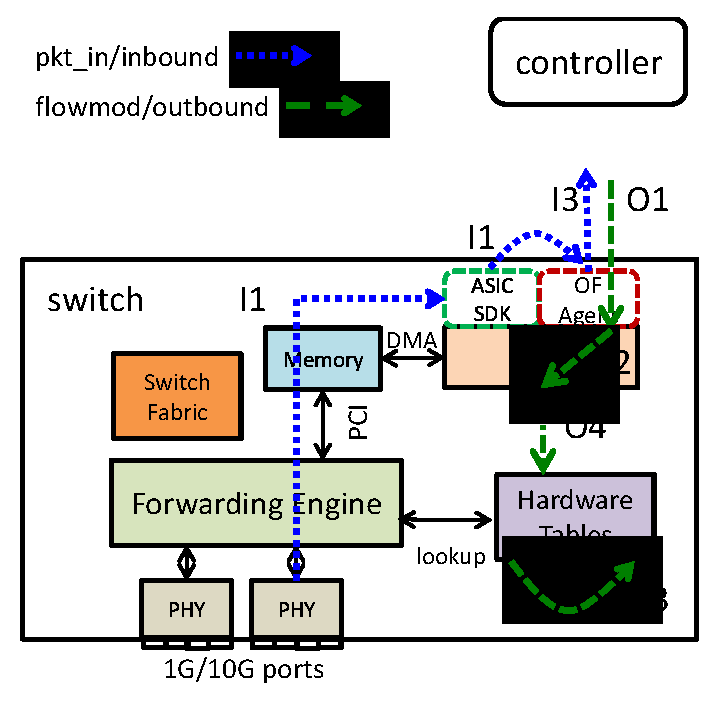
\epsfig{file=./figs/openflow_switch_illustrate.eps,width=0.4\textwidth} %%changed
\includegraphics[width=2.25in]{figs/openflow_switch.PNG}
\caption{Schematic of an OpenFlow switch. Different rectangular blocks indicate different components of a switch; 
different boxes do not mean different chips. We also show the factors contributing to inbound and outbound latency}\label{openflow_switch_delay}
%\vspace{-0.05in}
\end{figure}

{\bf \packetin\ processing: } When a packet arrives, the switch ASIC
first looks it up against the switch's hardware forwarding tables. If
a match is found, the packet is forwarded at line rate. Otherwise the
following steps take place (Figure~\ref{openflow_switch_delay}): (I1)
Switch ASIC decides to send the packet to the switch's CPU via the PCI/PCIe
bus. (I2) An OS interrupt is raised at which point the ASIC SDK gets
the packet and dispatches it to the switch-side openflow agent. (I3)
The agent wakes up, processes the packet, and sends to the controller
a \packetin\  message spanning the first 128B including header.
All of three steps, I1--I3,  can impact the latency in generating \packetin,
which we call {\em inbound   latency}. 

The application residing on the controller processes the message and
upon determining routes for packets belonging to the corresponding
flow, sends a \flowmod\ and a \packetout\ message. The \flowmod\
message describes the action the switch should apply to all future
packets of the flow: this could be forward according to some rule,
update an existing rule, or delete a rule. The format of a typical ``simple''
rule is \emph{srcip=A,dstip=B,action=output:3} (the rule can cover a total of 12 matching fields in Openflow 1.0); wild-cards can be used.
%\aditya{add here} 
The rule may also specify a priority (to
determine which rule to apply when multiple rules match a packet) and
a timeout after which the rule is deleted from the table. The
\packetout\ message simply releases the packets buffered at the switch
to be forwarded along.

%\li{The following does not parse. It also repeats lots of text from two
%  parapraphs before.}
{\bf \flowmod\ processing: }
When it receives a \flowmod, the switch takes the following steps: (O1) The
switch software running on the CPU parses the OpenFlow message. (O2) The
software schedules the rule to be  applied to hardware tables, typically  TCAM.
% \footnote{This involves a
%   write of the rules to hardware registers on the switch. The
%   processor may need to read (poll) another register on the switch
%   that tells it when the switch is ready to receive the next write.}.
(O3) Depending on the nature of the rule, the chip SDK may require
existing rules on the switch to be moved around, e.g., to accommodate
high priority rules. (O4) The hardware table is updated with the rule.
All of four steps O1--O4 impact the total delay in fully executing
\flowmod\ action, which we call {\em outbound delay}.

% The actions described above are generally applicable to different
% versions of OpenFlow. \aditya{correct? do we need to say more?}

% In this paper, we focus on the delays imposed at the switch. We ignore
% the impact of the propagation delay to the controller and control
% application processing itself. The latter is typically fast, while the
% former can be made negligible by careful placement of controller
% replicas. \marina{elastic controller placement paper}

SDN applications can be of two forms: {\em
  reactive} or {\em  proactive}. The former work by enforcing default-off
forwarding to flow sub-spaces; this causes any flow in that sub-space
to generate a \packetin\ event when it reaches an ingress switch for
the first time. The application then determines the forwarding action
and sends the corresponding \flowmod\ messages down to the
switch. These applications are impacted by both in- and outbound
delays. Proactive applications directly update network
forwarding state using \flowmod\ messages. They are mainly impacted by
outbound delays.%  (and possible interactions with inbound messages of
% other packets).

%\aditya{are we missing anything}

\subsection{Motivating Applications}

In what follows, we provide examples of management applications that
require fine-grained control over data plane state. We highlight the
impact of inbound and outbound latencies on the applications' objectives.

% A natural question that arises is whether that are scenarios where the
% latencies imposed by SDN switches during OpenFlow actions outlined
% above matter. In what follows, we described three SDN example
% scenarios to highlight the impact of latencies on the applications'
% overall performance.
 
% \emph{Inter-DC Traffic Engineering}
% XXX brief description of SWAN XXX

% A central challenge in systems such as SWAN is that fully using
% network capacity requires many forwarding rules at switches to exploit
% many alternative paths through the network. Furthermore, route updates
% in such systems invoke congestion-free update plans that leverage
% ``scratch'' capacity on network links to shift load from old to new
% paths in a gradual step-by-step fashion so as to not cause transient
% congestion that can hurt latency-sensitive traffic. Such update
% schemes consume additional rules in switches as well. 

% Unfortunately, commodity switches support a limited number of
% forwarding rules. To overcome this limitation, SWAN proposes
% dynamically changing, based on prevailing traffic patterns and demand,
% the set of paths available in the network. This may require updating
% the rules frequently.

% If such updates take longer, then there are two consequences: (a) Link
% utilization is reduced; (b) there might be congestion during the route
% updates XXX are we claiming here that SWAN assumes each stage is
% instantaneous XXX XXX also, need to be more concrete, with numbers XXX

% Traditionally, link of switch failures in networks
% were handled either by distributed routing or fast failover to backup
% paths. Distributed routing converges very slowly, resulting in link
% congestion or packet drops. Fast failover requires the reservation of
% dedicated link capacity. This results in low average link utilization,
% 30\%-40\%~\cite{B4}. SDN has the potential to bring the best of both
% worlds: quickly set up new paths without suffering from low link
% utilization.
% SWAN briefly mentions that link and switch failures are detected and reported to
% the controller. The controller in turn computes new allocations. SWAN does not
% provide details on how to setup the new paths. There can be significant amount
% of packet drops or congestion (if switch data plane redistributes traffic among
% remaining links). 

% \aditya{cut next two paras out?}

% Recent approaches for software-defined inter-DC
% wide-area networks, e.g., B4~\cite{B4} and~\cite{swan}, react to
% failures by pruning failed links or switches from route computations
% and ECMP groups. However, this does not guarantee that there will be
% no congestion. To address this issue, B4, for example, throttles low
% priority traffic to ensure no congestion for high priority traffic.
% This leads to low link utilization (50\% instead of 95\% during normal
% case~\cite{B4}) before a new traffic engineering allocation is
% installed. Thus, fast path setup upon failure can increase link
% utilization and avoid prolonged disruption to low priority traffic
% when failure happens in the DC WAN case.

% In settings other than DC WAN, such as a backbone network, there may
% not be enough low priority traffic to throttle to avoid congestion of
% high priority traffic considering that high priority video traffic
% makes up a substantial portion of traffic. Thus, fast path setup can
% be the only cost-effective means to minimize network disruption of
% applications.

{\bf Mobility: } Recent work~\cite{softcell} advocates using SDN to
simplify path setup and management in cellular networks. In these
settings, paths need to be set up whenever devices want to access the
Internet. In addition, these paths need to be reconfigured during
handoff. Currently these
paths are implemented as GPRS Tunneling Protocol (GTP) tunnels in LTE.
% A control plane entity, called Mobility Management Entity (MME),
% instructs base stations, serving gateways (S-GWs) and packet data
% network gateways (P-GWs) to setup tunnels from base stations to S-GWs,
% and from S-GWs to P-GWs. Recent efforts, e.g.,
% SoftCell~\cite{softcell}, have argued for replacing existing special
% purpose equipment used for S-GW and P-GWs with OpenFlow switches and
% leverage SDN to establish tunnels \aditya{say why, briefly}.
To avoid impacting the performance of subscribers, these tunnels must be setup
within a small latency bound. 
%\aditya{give a number.} 
%number is in the next paragraph
For example, when a mobile device in
idle state wants to communicate with an Internet server it needs first
to transition from idle state to connected state. According to recent
measurement studies~\cite{MorleyMobisys2012}, this transition delay is
around 260 ms in LTE. To keep access latency below 300 ms as
recommended by Web service providers, path setup must finish in 
40 ms. This can be very challenging especially when paths for multiple
devices need to be setup at once, e.g., during a popular event.
%  \aditya{why? is this trying to say
%   that installing path for a single flow can easily exceed 40ms? that
%   doesn't seem to be true}. % Similarly, during handoff, paths
% % must be reconfigured very fast to avoid throughput drop.

{\bf Failover: } % Traditionally, link or switch failures in networks
% were handled either by distributed routing or fast failover to backup
% paths. Distributed routing can take a long time to reconverge,
% resulting in transient loops, 
% congestion or packet drops. Fast failover techniques speed up this
% process, but they require the reservation of
% dedicated link capacity, so as to avoid congestion from failover
% traffic. Operators typically reserve nearly half of link
% capacities to this end~\cite{B4}. 
It is possible that SDN can help mitigate the network-wide impact of
failures in wide-area networks, reducing both downtime and congestion
without requiring significant over provisioning: when failures occur,
the SDN management application can quickly compute new paths for flows
traversing failed nodes or links, while also simultaneously rerouting
other high/low priority flows so as to avoid hot-spots~\cite{swan}.
However, this requires significant updates to network state at
multiple network switches. The longer this update takes, the longer
the effect of failure is felt in the form of congestion and drops. We
find that outbound latencies can inflate the time by nearly 20s
(\S\ref{s:evaluation}) putting into question SDN's applicability to
this scenario. 



\iffalse
There are three cases depending on the state of a mobile device (referred as UE
typically). (1) A UE wants to communicate 
in idle state. (2) In the connected state, a UE's application triggers
dedeciated connection setup. (3) A UE's connection needs to be
reconfigured during handoff. According to measurement
studies~\cite{MorleyMobisys2012}, the transition delay from idle to
connected for a UE is 260ms in LTE. Therefore, to keep the total
latency below 300ms as recommended by web service providers, path setup
has to be fast. Even though paths during handoff can be done in a
make-before-break fashion, in many settings there may not be enough
prior time for the network to respond. The first case is the most
challenging. \aditya{this scenario is a bit all over the place and
  hard to follow} 
%\marina{May be presenting this scenario as an adaptive radio
%  network backhaul with time varying demands from the cellular nw would be
%  easier} 
% that will take too much space to describe the problem; not much different from
% microte. 
\fi

% Outbound latencies can directly impact various {\em consistent update
%   primitives} used within management applications. Examples include
% one-shot updates~\cite{consistentupdates}, congestion-, drop-, or
% loop-free updates~\cite{swan,mahajan13:hotnets}, etc. Depending on the
% size of the network, and the nature of updates, the impact can be
% significant and can hurt the application. We show this qualitatively
% and quantitatively for one-shot updates in Sections XXX and XXX.

{\bf Intra-DC Traffic Engineering:} Some recent proposals, such as
MicroTE~\cite{microte} and Hedera~\cite{hedera} have argued for using
SDN to route traffic subsets at fine time-scales in order to achieve
fine-grained traffic engineering in data centers. For instance,
MicroTE leverages the fact that a significant fraction of ToR-to-ToR
DC traffic (ToR is ``top-of-rack'' switch) is predictable on short
time-scales of a 1-2s. It computes and installs at ToR switches
routes for such traffic on short
time-scales. % The computed routes may only be effective for 1-2s
% after which a new sets of routes may be more optimal. 
Thus, latencies in installing routes can significantly undermine
MicroTE's effectiveness. Indeed, we find that updating a set of routes
at a ToR switch in MicroTE can take as long as 0.5s on some SDN switches
(\S\ref{s:evaluation}). 

% \times T$s, $n$ is the number of destination ToRs and $T$ is the latency to
% install any give rule. Our measurements presented later in the section
% show the $T \approx 2$ms, so this can be as high as 1s for a
% network with 500 ToR switches. \marina{ref for this number 500 ToR sw} This is significant given that traffic
% predictability may only last for 1-2s. \aditya{more to say here?}

% Hedera makes scheduling and rerouting decisions as often as every few
% seconds for flows exceeding 100MB. However, even such ``elephant''
% flows last a few seconds at most. In some situations, routes for many
% such flows may need to be installed at once at a switch; e.g., when
% many tasks placed in a rack shuffle large intermediate results to
% tasks in other racks, or during data read or data ingest operations in
% big data jobs~\cite{orchestra}. The resulting latency can inflate the
% flows' completion times, and in turn impact job-level performance.


% For path setup from IDLE to CONNECTED, promotion delay is 260ms according to
% Morley's paper. Would this make the path setup not the bottleneck?
% what about voLTE?


% LocalWords:  Intra MicroTE wrt ECMP eval Reactiveness msec Failover handoff
% LocalWords:  SDN GTP LTE GWs GW SoftCell OpenFlow

